\documentclass[10pt]{beamer}
\usetheme{Warsaw}

\setbeamertemplate{footline}{}
\setbeamersize{text margin left=3.5mm,text margin right=3.5mm} 

\usepackage{hyperref}
\hypersetup{
    colorlinks=true,
    linkcolor=blue,
    filecolor=magenta,      
    urlcolor=blue,
}
 
\urlstyle{same}

\usepackage{datetime}
\newdateformat{specialdate}{\twodigit{\THEDAY}.\twodigit{\THEMONTH}.\THEYEAR}

\usepackage[utf8]{inputenc}

\usepackage{float}
\usepackage{graphicx}
\graphicspath{ {./images/} }

\usepackage{verbatim}

\usepackage{caption}
\captionsetup[figure]{name=Fig.}


\title{Benchmark comparison of protein sequence preprocessing effect on learning task for Pfam family classification}
\author{Maciej Sikora}

\begin{document}
\frame{\titlepage}


\begin{frame}
\frametitle{Inspiration and problem overview}
\begin{itemize}
\item \textbf{Data preprocessing for size reduction without losing crucial information.}
\end{itemize}

\begin{itemize}
\item A growing amount of biological data.
\item Full Swissprot database:  $>$250 MB
\item Full Uniprot database: around 10 GB
\item Combining data from other databases would increase those numbers even more.
\item The analysis becomes much harder and time-consuming
\end{itemize}
\end{frame}

\begin{frame}
\frametitle{Inspiration and problem overview}
\begin{itemize}
\item \textbf{Data preprocessing for size reduction without losing crucial information.}
\end{itemize}

\begin{itemize}
\item 0.25\% sequences manually annotated in Uniprot
\item Automated data annotating
\item Need for better models
\item More complicated models take longer to train
\end{itemize}
\end{frame}

\begin{frame}
\frametitle{Biovec}
\begin{itemize}
\item Biovec [1][2] -- a multidisciplinary model combining knowledge from biology, linguistics and statistics.
\item Analysis of k-mers in a bigger sequential context.
\item Calculating vectors of the probability of k-mers in the given context.
\item Using preprocessed metadata for training.
\end{itemize}
\begin{figure}[H]
\begin{center}
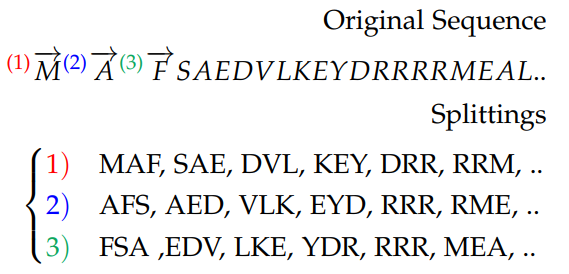
\includegraphics[width=0.5\textwidth]{biovec}
\end{center}
\end{figure}
\end{frame}

\begin{frame}
\frametitle{Compared methods of preprocessing}
\begin{itemize}
\item Data source: Swissprot -- manually reviewed part of the Uniprot[3] database
\item Filtering by most frequent organisms and families
\item CD-HIT[4] -- removing very similar protein sequences
\item Padding
\item Splitting to stratified train and test pools
\item Shuffling
\end{itemize}

\begin{itemize}
\item Original
\item Singletons -- dtype int8
\item Triplets -- dtype int16
\item Biovec
\end{itemize}
\begin{figure}[H]
\begin{center}
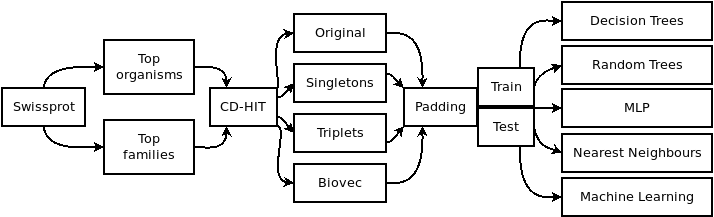
\includegraphics[width=0.8\textwidth]{workflow}
\end{center}
\end{figure}
\end{frame}

\begin{frame}
\frametitle{Tested models}
\begin{itemize}
\item Decision trees
\item Random trees
\item MLP
\item Nearest neighbours
\item Machine Learning (Simple Dense model)
\end{itemize}

\begin{itemize}
\item Grid Search for optimal parameters
\item Cross-validation
\end{itemize}
\begin{figure}[H]
\begin{center}
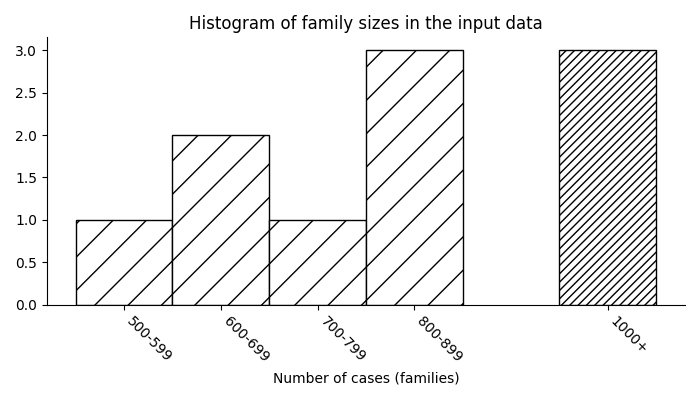
\includegraphics[width=0.7\textwidth]{histogram}
\end{center}
\end{figure}
\end{frame}

\begin{frame}
\frametitle{Results}
\begin{figure}[H]
\begin{center}
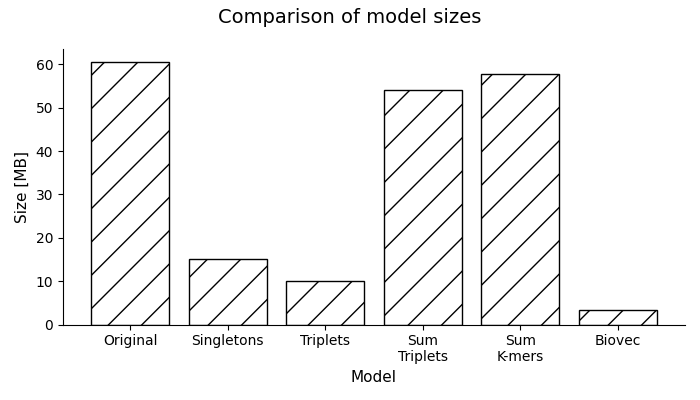
\includegraphics[width=0.5\textwidth]{sizes}
\end{center}
\end{figure}

\begin{figure}[H]
\begin{center}
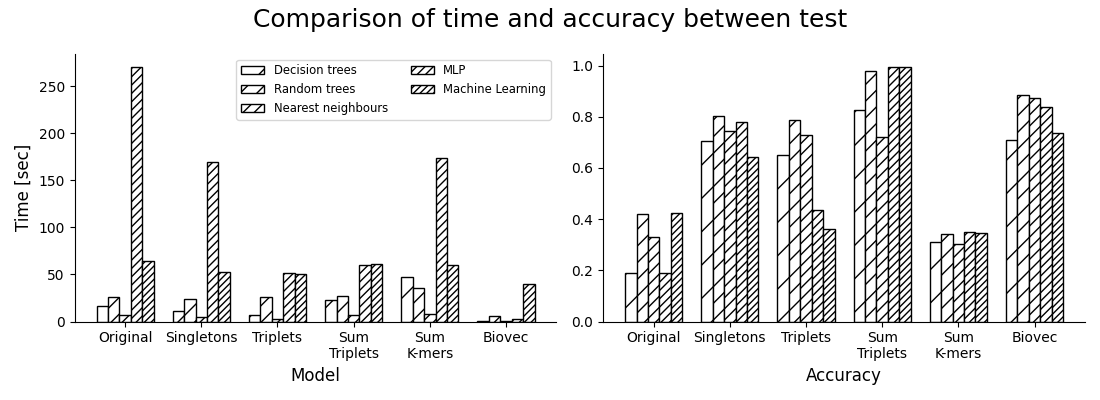
\includegraphics[width=0.9\textwidth]{benchmark}
\end{center}
\end{figure}
\end{frame}



\begin{frame}
\frametitle{Summary}
\begin{itemize}
\item Treating protein data as string objects might have a negative impact on the training process.
\item Simple conversion to numerical data improves both accuracy  and runtime.
\item Further numerical categorization for triplets while speeding up the learning process is losing some of the information leading to decreased accuracy.
\item The neighbourhood of amino acids can be analysed using a more sophisticated biovec model.
\item Biovec yields both better results and up to 100 times faster training process (MLP) compared to the original model.
\item Biovec model data weighs over 20 times less than the original one.
\end{itemize}
\end{frame}

\begin{frame}
\frametitle{References}
\begin{footnotesize}
\begin{enumerate}
\item Article Source: Continuous Distributed Representation of Biological Sequences for Deep Proteomics and Genomics
\item https://gitlab.com/victiln/protvec
Asgari E, Mofrad MRK (2015) Continuous Distributed Representation of Biological Sequences for Deep Proteomics and Genomics. PLOS ONE 10(11): e0141287. https://doi.org/10.1371/journal.pone.0141287
\item The UniProt Consortium, UniProt: the universal protein knowledgebase in 2021, Nucleic Acids Research, Volume 49, Issue D1, 8 January 2021, Pages D480–D489, https://doi.org/10.1093/nar/gkaa1100
\item Li W, Godzik A. Cd-hit: a fast program for clustering and comparing large sets of protein or nucleotide sequences. Bioinformatics. 2006 Jul 1;22(13):1658-9. doi: 10.1093/bioinformatics/btl158. Epub 2006 May 26. PMID: 16731699.
\end{enumerate}
\end{footnotesize}
\end{frame}
\end{document}